\documentclass[a4paper,10pt]{article}
\usepackage[utf8]{inputenc}
\usepackage[english,russian]{babel}
\usepackage[top=2cm,bottom=3cm,left=0.5cm,right=2cm,nohead]{geometry}
\usepackage{multicol}
\usepackage{graphicx}

\graphicspath{{images/}}

\begin{document}
\section*{задачи с экзаменов и Бородаченковой}
    5 команд значит 5 инструкций число строк макроса неважно, что такое макрорасширение найдёте в файлах ответы к экзаменам искать там где экзамены писать на листочке\\
    \begin{figure}[htbp]
        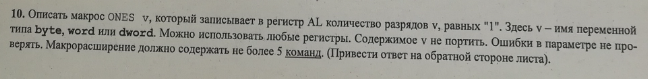
\includegraphics[width=0.85\textwidth]{Ones.png}
        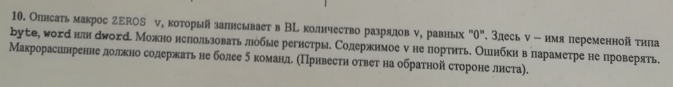
\includegraphics[width=0.85\textwidth]{Zeros.png}
        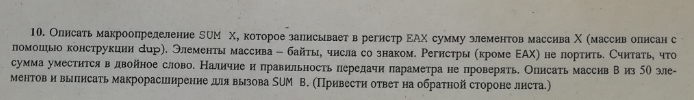
\includegraphics[width=0.85\textwidth]{SUM.png}
        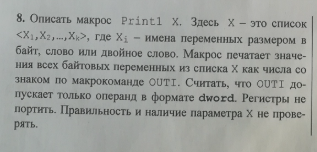
\includegraphics[width=0.65\textwidth]{Print1.png}
    \end{figure}
    посмотреть файл Задачи 10\_шпора \\
    экзамен давний некоторые ещё времён 16 битного ассемблера, подсказка использовать @substr(строка, начало[, длина]) строка начинается с 1
    \begin{figure}[htbp]
        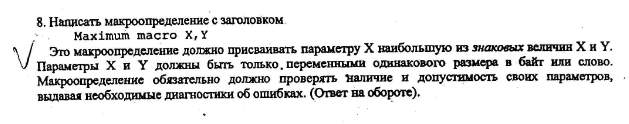
\includegraphics[width=0.85\textwidth]{Maximum.png}
        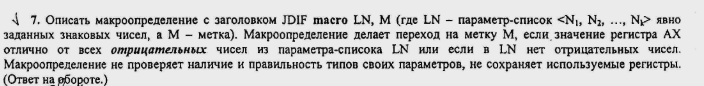
\includegraphics[width=0.85\textwidth]{JDIF.png}
        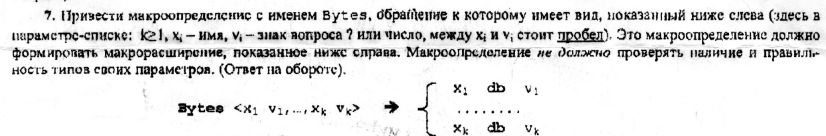
\includegraphics[width=0.85\textwidth]{Bytes.png}
    \end{figure}
    если задач недостаточно то таких номеров в сборнике найти можно много \\
\end{document}